% =====================================================================================
% ICTDS — Lab Report: Milestone 1
% Course: Introduction to Computational Thinking and Data Science (NOVA IMS)
% Instructor: Paulo Souza
% Group 11 — Climate Stability Analysis: Bragança vs Viseu
% =====================================================================================

\documentclass[11pt,a4paper]{article}

\usepackage[margin=1in]{geometry}
\usepackage{graphicx}
\usepackage{float}
\usepackage{booktabs}
\usepackage{amsmath}
\usepackage{amssymb}
\usepackage{hyperref}
\usepackage{xcolor}
\usepackage{caption}
\usepackage{multirow}
\usepackage{array}
\usepackage{longtable}

\hypersetup{
  colorlinks=true,
  linkcolor=black,
  urlcolor=blue,
  citecolor=blue
}

\newcommand{\CourseName}{Introduction to Computational Thinking and Data Science (ICTDS)}
\newcommand{\AcademicYear}{2025/2026}
\newcommand{\LabNumber}{Milestone 1}
\newcommand{\LabTitle}{Climate Stability Analysis: Bragança vs Viseu}
\newcommand{\GroupID}{Group 11}
\newcommand{\DateSubmitted}{\today}

\begin{document}

\begin{center}
  {\Large \textbf{\CourseName}}\\
  {\small Academic Year: \AcademicYear}\\[0.2cm]
  {\Large \textbf{\LabNumber: \LabTitle}}\\[0.3cm]
\end{center}

\noindent
\textbf{Group:} \GroupID \hfill \textbf{Submitted:} \DateSubmitted\\[0.2cm]
\noindent
\textbf{Members:}
\begin{itemize}
  \item 20250873 — Aakarshak Asiwal \textit{(Leader)}
  \item 20250013 — Mozhdeh Marvi
  \item 20251273 — Fakhar Mahmood Khan
  \item 20251224 — Fatima Zahra
  \item 20251218 — Bohair Hameed
  \item 20241794 — Rodrigo Souta
\end{itemize}
\rule{\textwidth}{0.4pt}

% =====================================================================================
\section{Introduction}
% =====================================================================================

\textbf{Goal:} This report presents a comparative climate stability analysis of two Portuguese cities — Bragança and Viseu — to determine which location is better suited for a \textbf{cold-storage logistics facility}. The analysis spans daily meteorological data from 2018 to 2025, evaluating temperature distributions, seasonal variability, extreme weather events, and the thermal load experienced at each site. The key question is: \textit{Which city offers a more stable, cooler, and operationally predictable climate?}

% =====================================================================================


\section{Dataset Description}


% =====================================================================================

\subsection{Data Source and Scope}

Two CSV datasets were used — \texttt{raw\_BRAGANCA.csv} and \texttt{raw\_VISEU.csv} — each containing daily observations. After removing the redundant \texttt{time} column and excluding the incomplete year 2026, both datasets span \textbf{2018-01-01 to 2025-12-31}, yielding \textbf{2,922 daily records per city}.

\newpage

\subsection{Variables}

The following features were available or derived from the raw data:

\begin{table}[H]
\centering
\caption{Dataset Variables}
\begin{tabular}{lll}
\toprule
\textbf{Variable} & \textbf{Type} & \textbf{Description} \\
\midrule
\texttt{temperature\_2m\_max} & Numerical & Daily maximum temperature at 2m (°C) \\
\texttt{temperature\_2m\_min} & Numerical & Daily minimum temperature at 2m (°C) \\
\texttt{temperature\_2m\_mean} & Numerical & Daily mean temperature at 2m (°C) \\
\texttt{precipitation\_sum} & Numerical & Total daily precipitation (mm) \\
\texttt{wind\_speed\_10m\_max} & Numerical & Max wind speed at 10m (km/h) \\
\texttt{wind\_gusts\_10m\_max} & Numerical & Max wind gusts at 10m (km/h) \\
\texttt{shortwave\_radiation\_sum} & Numerical & Daily solar radiation sum (MJ/m²) \\
\texttt{sunshine\_duration\_hrs} & Derived & Sunshine duration (hours; converted from seconds) \\
\texttt{relative\_humidity\_2m\_mean} & Numerical & Mean relative humidity at 2m (\%) \\
\texttt{cloudcover\_mean} & Numerical & Mean cloud cover (\%) \\
\texttt{day\_length\_hrs} & Derived & Length of day in hours (sunset $-$ sunrise) \\
\texttt{DTR} & Derived & Diurnal Temperature Range = max $-$ min (°C) \\
\bottomrule
\end{tabular}
\end{table}

\subsection{Data Cleaning and Preprocessing}

\begin{itemize}
  \item The redundant \texttt{time} column was dropped.
  \item The \texttt{date} column was converted to datetime; \texttt{year} and \texttt{month} columns were extracted.
  \item \texttt{sunshine\_duration} was converted from seconds to hours.
  \item \texttt{day\_length\_hrs} was derived from sunset and sunrise timestamps; those columns were subsequently dropped.
  \item Data from year 2026 was excluded as it only covered January–February, which would introduce seasonal bias.
  \item A \texttt{season} categorical variable was created: \textit{Winter} (Dec–Feb), \textit{Spring} (Mar–May), \textit{Summer} (Jun–Aug), \textit{Autumn} (Sep–Nov).
\end{itemize}

The seasonal approach was chosen over yearly or monthly grouping: yearly grouping conflates opposite temperature regimes, while monthly grouping produces 12 categories — too granular for a summary analysis.

% =====================================================================================
\section{Methodology}
% =====================================================================================

\subsection{Main Questions}

\begin{itemize}
  \item Which city has lower mean temperatures across all seasons?
  \item Which city experiences fewer extreme heat days ($\geq$25°C, $\geq$30°C, $\geq$35°C)?
  \item Which city has a more stable temperature regime (lower DTR, lower inter-annual variability)?
  \item Which meteorological features most strongly correlate with temperature and thermal stability?
  \item How many anomalous temperature days does each city experience per season?
\end{itemize}

\subsection{Analysis Approach}

The analysis followed these steps:

\begin{enumerate}
  \item \textbf{Data loading and cleaning} — removal of redundancies, unit conversions, and feature derivation (DTR, day length, sunshine hours).
  \item \textbf{Seasonal categorization} — assigning each record to one of four seasons and excluding the partial year 2026.
  \item \textbf{Summary statistics} — computing mean, standard deviation, coefficient of variation (CoV), median, min, max, and IQR for all features, grouped by season, for both cities.
  \item \textbf{Temperature Stability Index} — constructing a composite index from three normalized components: within-season SD, mean DTR, and inter-annual CoV of seasonal mean temperature.
  \item \textbf{Pearson correlation analysis} — measuring linear relationships between eight meteorological features and three targets: mean temperature, DTR, and the Stability Index.
  \item \textbf{Extreme event detection} — using seasonal IQR fences ($Q_1 - 1.5 \cdot \text{IQR}$, $Q_3 + 1.5 \cdot \text{IQR}$) to flag anomalous temperature days.
  \item \textbf{Thermal envelope analysis} — computing monthly mean max, mean, and min temperatures to visualize the annual temperature profile.
  \item \textbf{Positive deviation analysis} — measuring deviations of daily max temperature above the monthly mean max, and counting high-temperature threshold exceedances.
\end{enumerate}

% =====================================================================================
\section{Results}
% =====================================================================================

\subsection{Summary Statistics — Temperature}

Table~\ref{tab:temp_summary} presents the seasonal mean temperatures and standard deviations for both cities.

\begin{table}[H]
\centering
\caption{Seasonal Mean Daily Temperature (°C) — Bragança vs Viseu (2018–2025)}
\label{tab:temp_summary}
\begin{tabular}{lcccccccc}
\toprule
 & \multicolumn{2}{c}{\textbf{Winter}} & \multicolumn{2}{c}{\textbf{Spring}} & \multicolumn{2}{c}{\textbf{Summer}} & \multicolumn{2}{c}{\textbf{Autumn}} \\
\cmidrule(lr){2-3}\cmidrule(lr){4-5}\cmidrule(lr){6-7}\cmidrule(lr){8-9}
\textbf{City} & Mean & SD & Mean & SD & Mean & SD & Mean & SD \\
\midrule
Bragança & 6.07 & 2.89 & 11.28 & 4.19 & 21.14 & 3.92 & 13.61 & 4.70 \\
Viseu    & 8.41 & 2.70 & 12.91 & 4.03 & 21.49 & 4.03 & 15.30 & 4.55 \\
\bottomrule
\end{tabular}
\end{table}

Bragança is consistently cooler than Viseu in every season. The temperature gap is most pronounced in \textbf{Winter} (2.34°C difference) and \textbf{Autumn} (1.69°C difference). Summer means are very close (21.14°C vs 21.49°C), while the spread (SD) is comparable across all seasons.

\subsection{Diurnal Temperature Range (DTR)}

Table~\ref{tab:dtr_summary} shows the seasonal mean DTR for both cities.

\begin{table}[H]
\centering
\caption{Seasonal Mean Diurnal Temperature Range — DTR (°C)}
\label{tab:dtr_summary}
\begin{tabular}{lcccc}
\toprule
\textbf{City} & \textbf{Winter} & \textbf{Spring} & \textbf{Summer} & \textbf{Autumn} \\
\midrule
Bragança & 7.82 & 10.50 & 12.95 & 9.33 \\
Viseu    & 7.75 & 9.83  & 12.87 & 8.99 \\
\bottomrule
\end{tabular}
\end{table}

DTR values are broadly similar across cities. Bragança shows slightly higher DTR in Spring and Autumn, indicating marginally wider daily temperature swings in those seasons.

\subsection{Temperature Stability Index}

The Stability Index was computed as the mean of three normalized components: within-season SD, mean DTR, and inter-annual CoV. A higher index indicates greater stability.

\begin{table}[H]
\centering
\caption{Temperature Stability Index by Season (0–1 scale; higher = more stable)}
\label{tab:stability}
\begin{tabular}{lcccc}
\toprule
\textbf{City} & \textbf{Winter} & \textbf{Spring} & \textbf{Summer} & \textbf{Autumn} \\
\midrule
Bragança & 0.260 & 0.200 & 0.238 & 0.293 \\
Viseu    & 0.374 & 0.241 & 0.216 & 0.333 \\
\bottomrule
\end{tabular}
\end{table}

Viseu scores higher in Winter and Autumn stability. However, \textbf{Bragança scores slightly higher in Summer} (0.238 vs 0.216), which is the most operationally critical season for a cold-storage facility. The indices are modest across both cities, reflecting that Portuguese climate carries meaningful seasonal variability.

\subsection{Pearson Correlations with Temperature Targets}

Table~\ref{tab:corr} summarizes the Pearson correlations between the eight meteorological features and mean daily temperature (T\textsubscript{mean}), DTR, and Stability Index.

\begin{table}[H]
\centering
\caption{Pearson Correlations: Features vs Temperature Targets (averaged across both cities)}
\label{tab:corr}
\begin{tabular}{lccc}
\toprule
\textbf{Feature} & \textbf{T\textsubscript{mean}} & \textbf{DTR} & \textbf{Stability Index} \\
\midrule
Sunshine Duration (hrs) & +0.57 & +0.77 & $-0.44$ \\
Shortwave Radiation (MJ/m²) & +0.73 & +0.80 & $-0.59$ \\
Cloud Cover (\%) & $-0.35$ & $-0.69$ & +0.12 \\
Relative Humidity (\%) & $-0.64$ & $-0.78$ & +0.27 \\
Precipitation (mm) & $-0.17$ & $-0.49$ & +0.10 \\
Wind Speed Max (km/h) & $-0.05$ & $-0.31$ & $-0.06$ \\
Wind Gusts Max (km/h) & $-0.02$ & $-0.31$ & $-0.09$ \\
Day Length (hrs) & +0.72 & +0.54 & $-0.72$ \\
\bottomrule
\end{tabular}
\end{table}

The strongest positive drivers of temperature and DTR are \textbf{solar radiation}, \textbf{sunshine duration}, and \textbf{day length}. Relative humidity and cloud cover show the strongest negative associations. Day length is particularly notable: it has the highest correlation with Stability Index ($r \approx -0.72$ for Viseu, $r \approx -0.55$ for Bragança), indicating that longer days are associated with lower thermal stability — consistent with higher summer variability.

\begin{figure}[H]
\centering
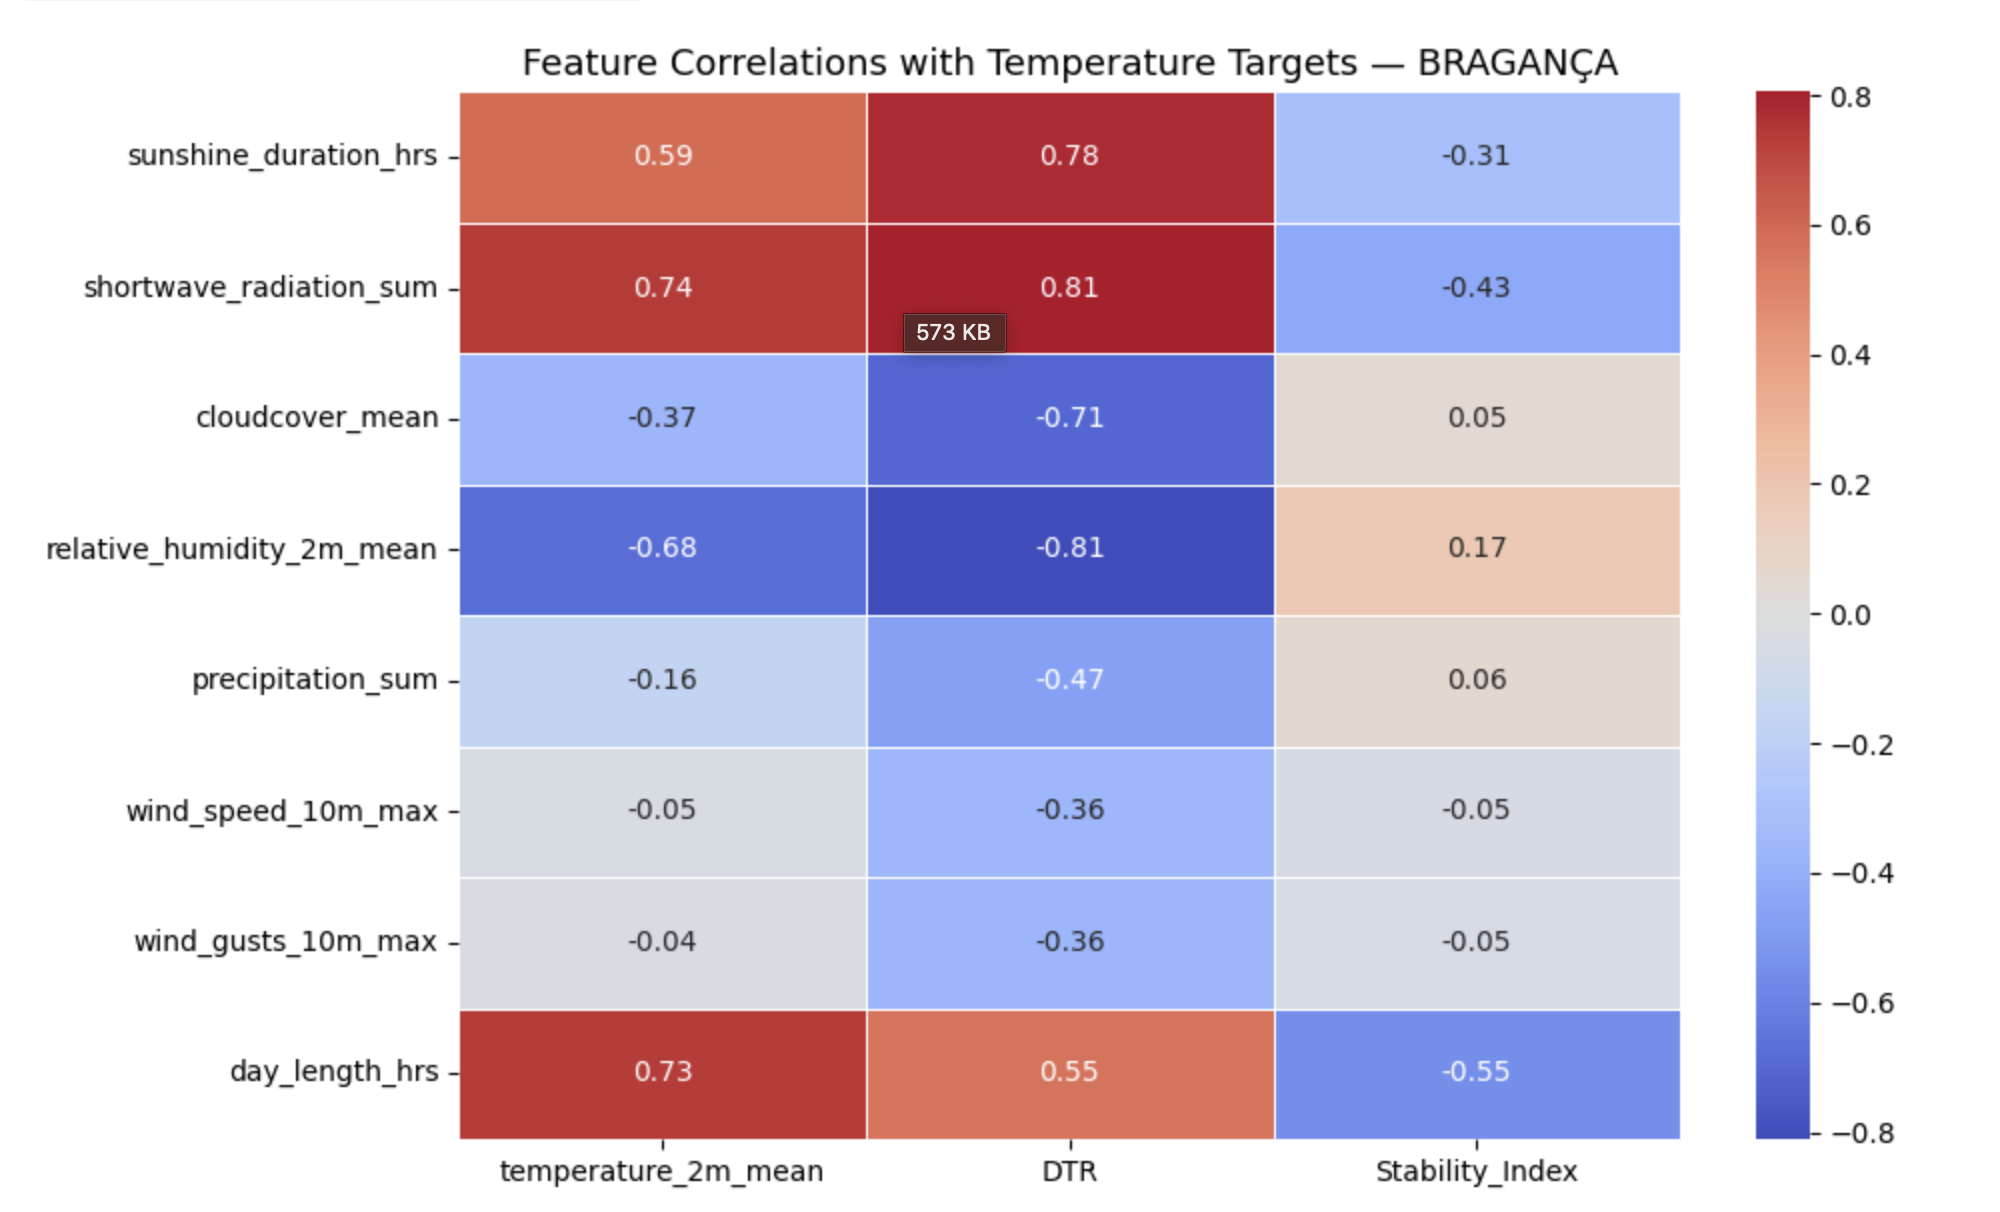
\includegraphics[width=0.85\textwidth]{corrBranganca.png}
\caption{Feature correlation heatmap with temperature targets — Bragança}
\label{fig:corr_br}
\end{figure}

\begin{figure}[H]
\centering
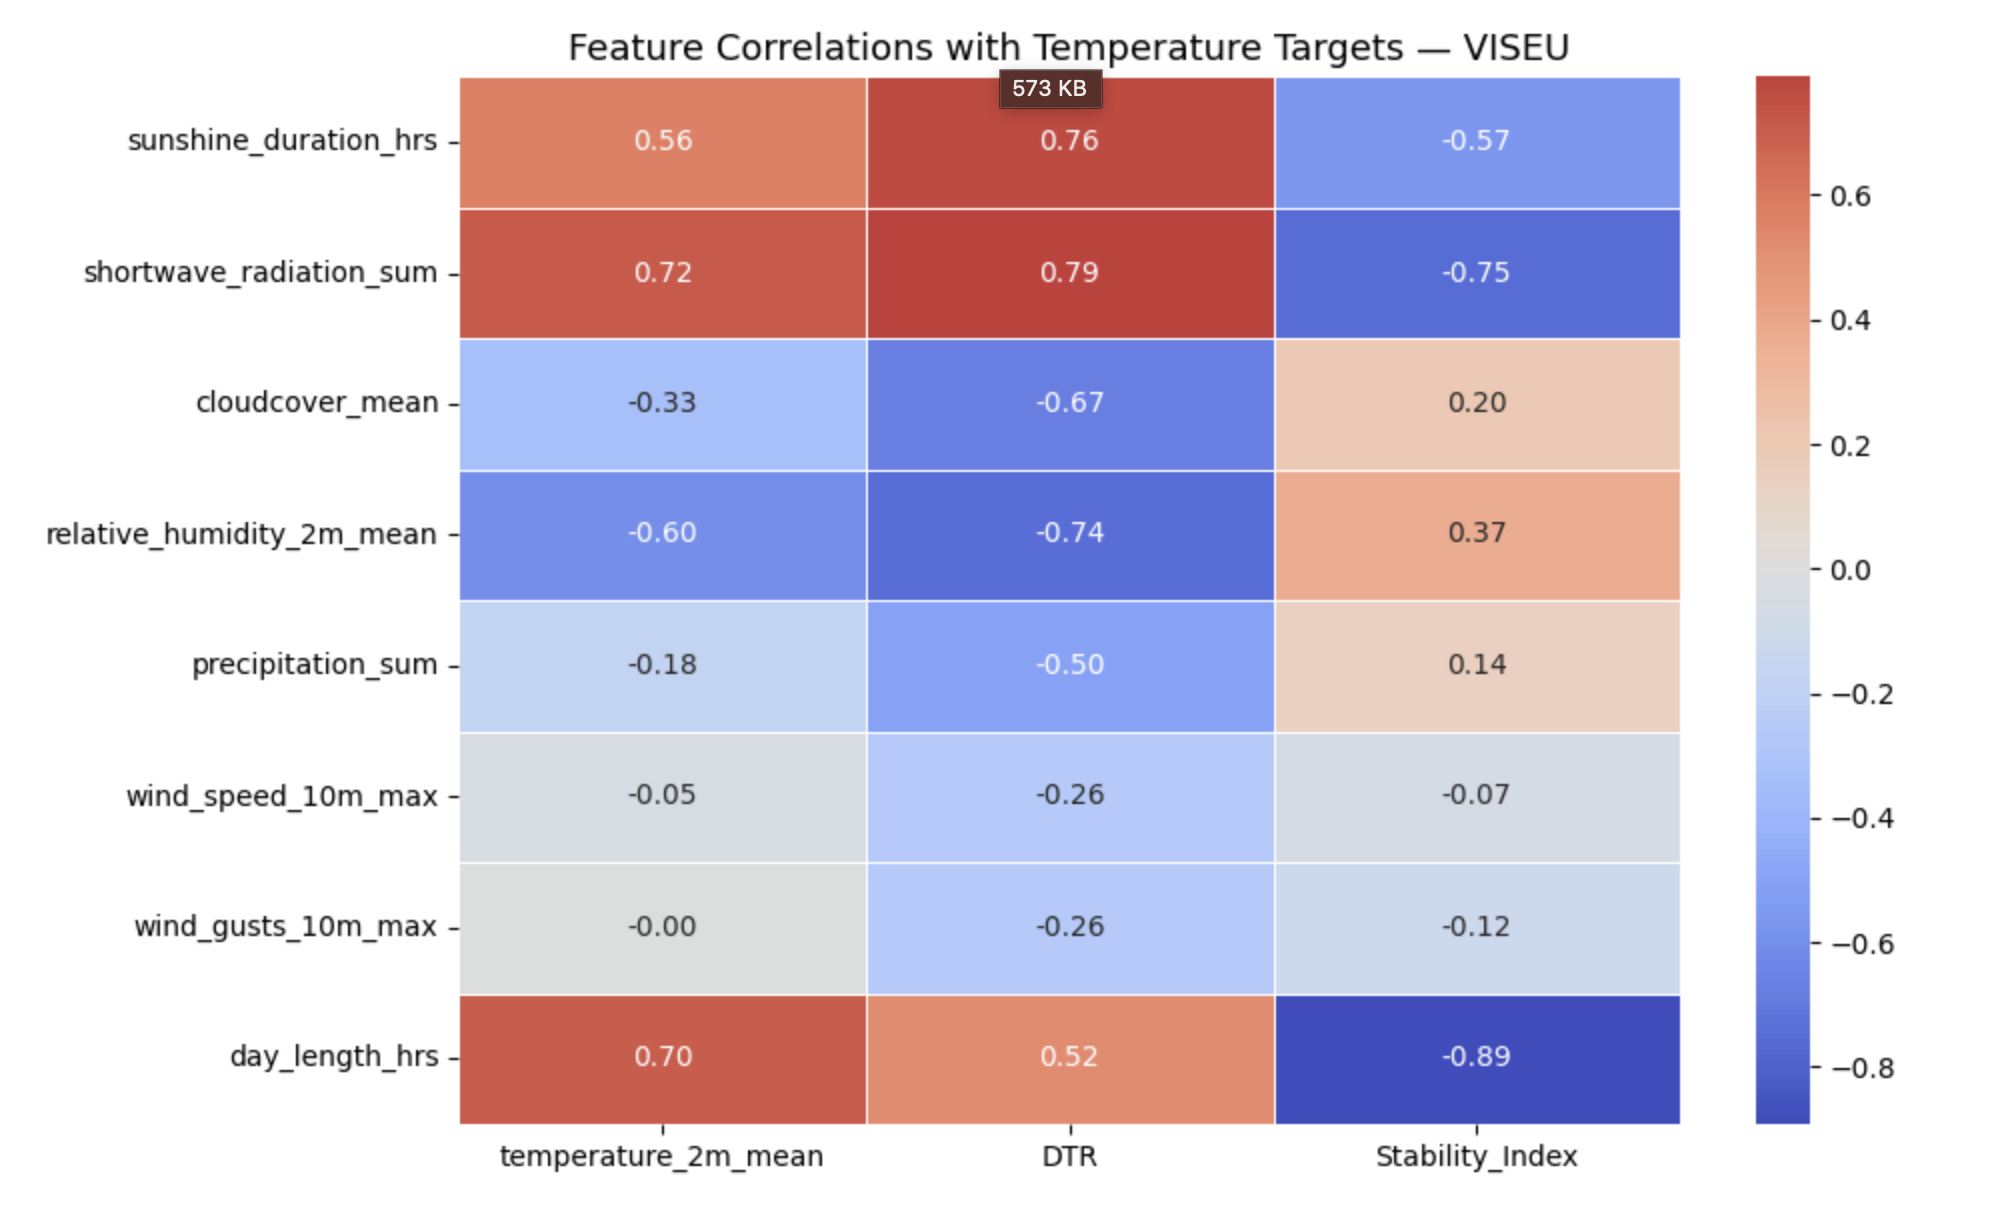
\includegraphics[width=0.85\textwidth]{CorrViseu.png}
\caption{Feature correlation heatmap with temperature targets — Viseu}
\label{fig:corr_vi}
\end{figure}

\subsection{Extreme Temperature Events}

Seasonal IQR fences were used to detect anomalous days. Results are summarized in Table~\ref{tab:extreme}.

\begin{table}[H]
\centering
\caption{Extreme Temperature Events by Season}
\label{tab:extreme}
\begin{tabular}{lcccccc}
\toprule
\textbf{City} & \textbf{Total} & \textbf{Winter} & \textbf{Spring} & \textbf{Summer} & \textbf{Autumn} \\
\midrule
Bragança & 7 & 0 & 6 & 1 & 0 \\
Viseu    & 6 & 0 & 3 & 1 & 2 \\
\bottomrule
\end{tabular}
\end{table}

Bragança has 7 extreme days vs Viseu's 6. The bulk of Bragança's extremes occur in Spring (6 events), while Viseu distributes across Spring and Autumn. On extreme days, both cities show markedly lower humidity, higher solar radiation, and higher DTR compared to normal days, indicating hot and dry anomalous events.

\begin{figure}[H]
\centering
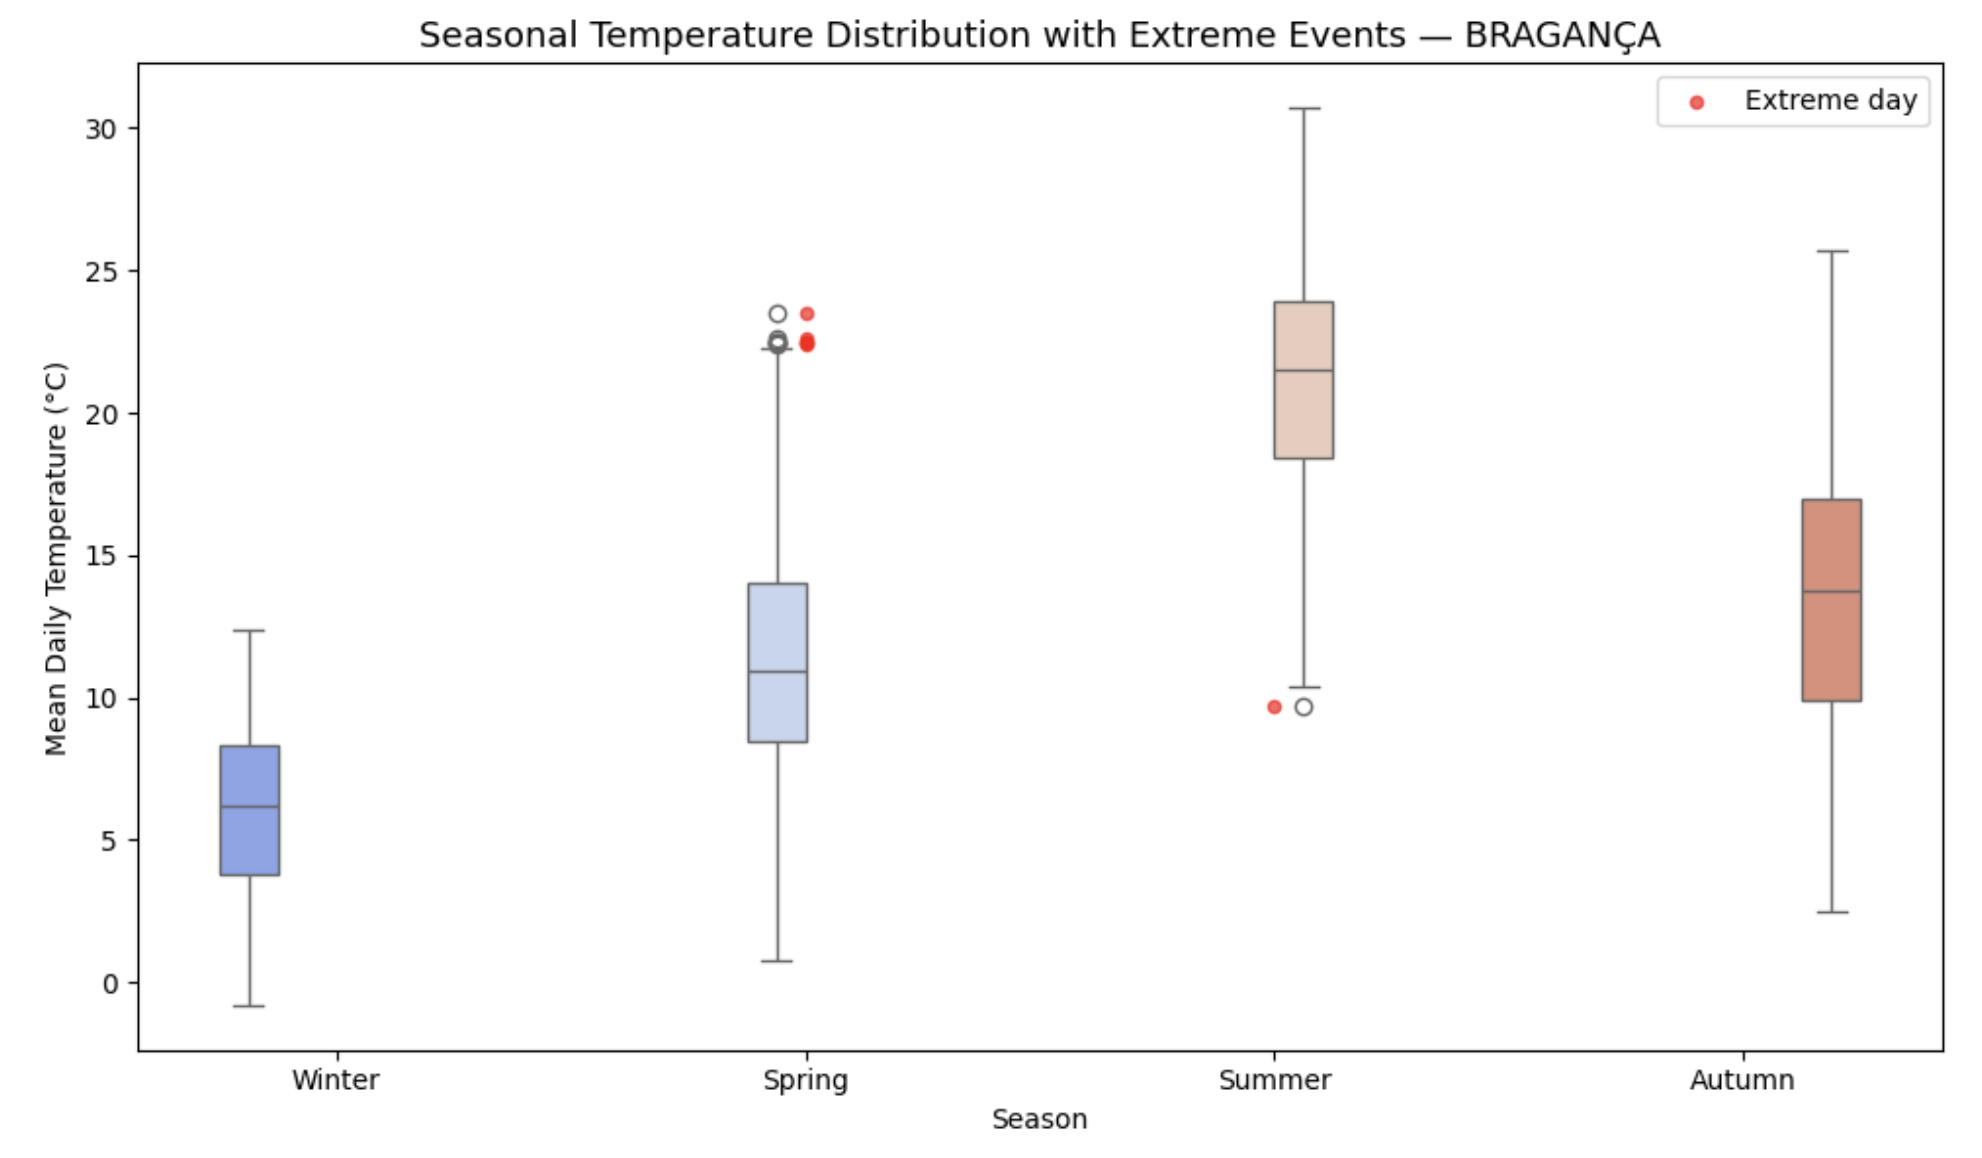
\includegraphics[width=0.85\textwidth]{extremeBrag.png}
\caption{Seasonal temperature distribution with extreme events highlighted — Bragança}
\label{fig:extreme_br}
\end{figure}

\begin{figure}[H]
\centering
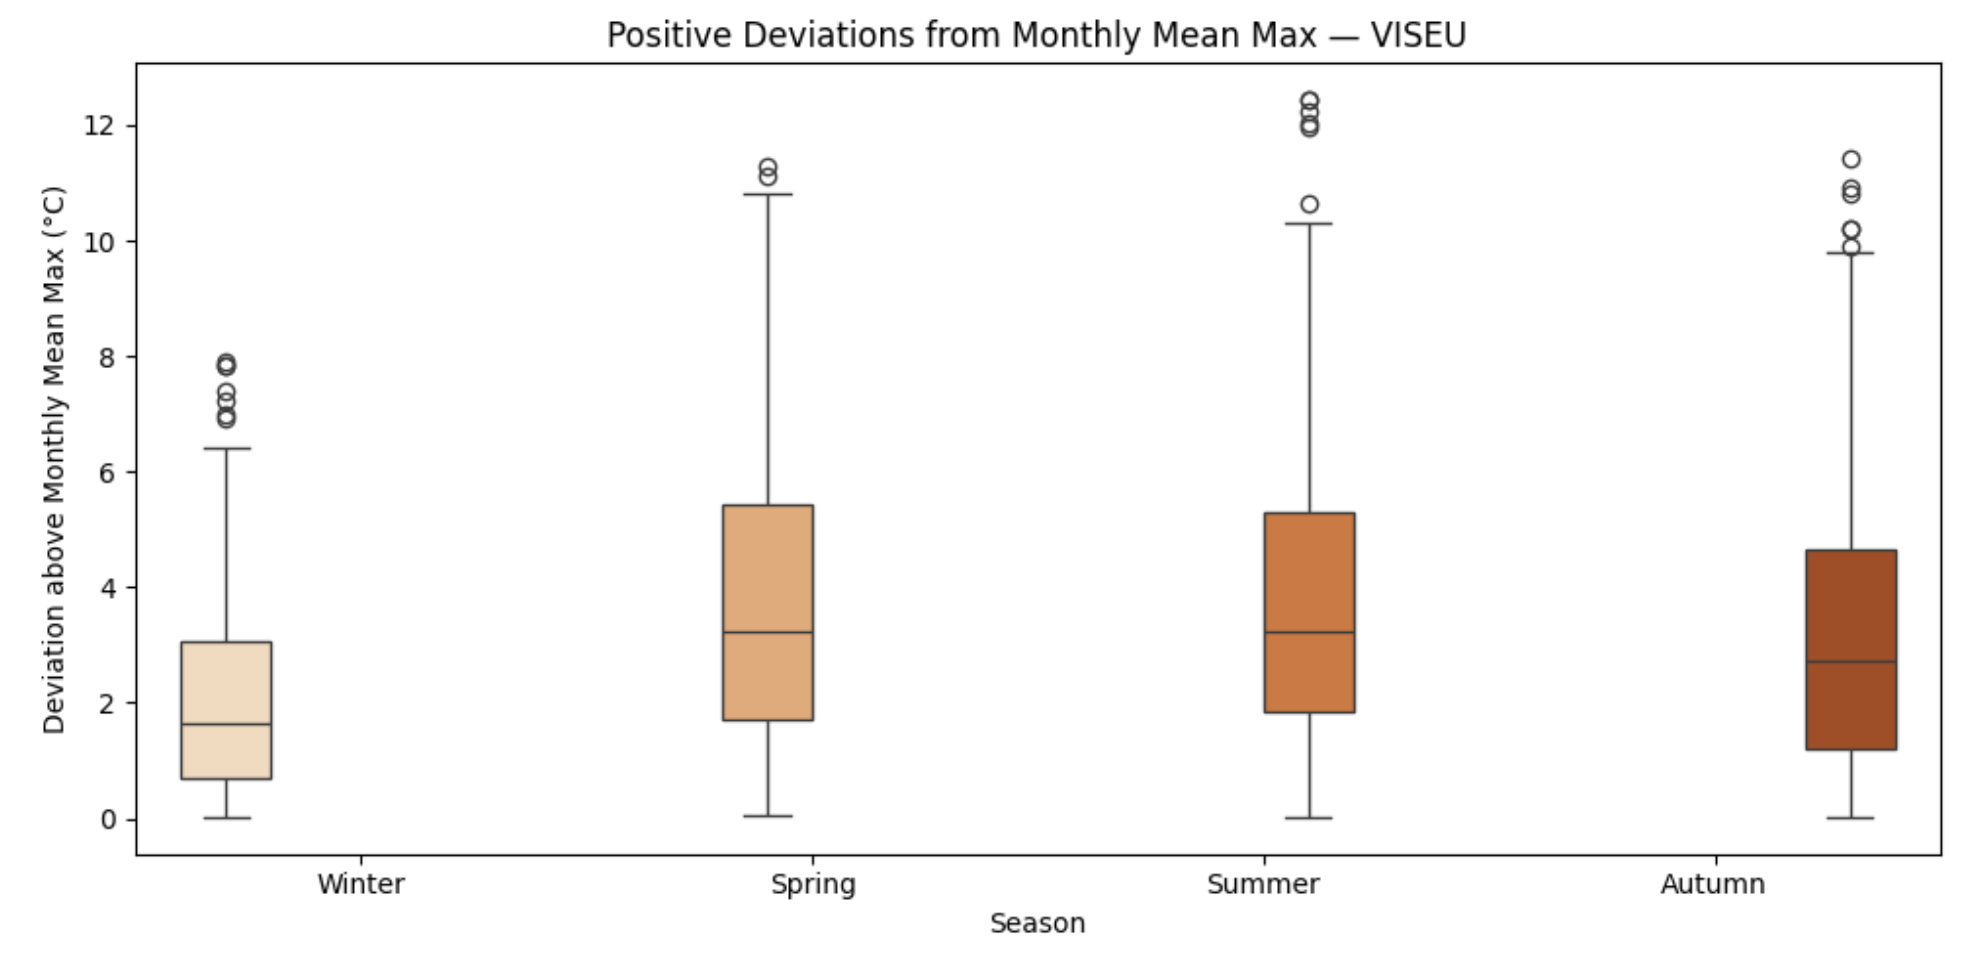
\includegraphics[width=0.85\textwidth]{extrViseu.png}
\caption{Seasonal temperature distribution with extreme events highlighted — Viseu}
\label{fig:extreme_vi}
\end{figure}

\subsection{High-Temperature Day Frequency}

\begin{table}[H]
\centering
\caption{Frequency of High-Temperature Days (2018–2025)}
\label{tab:hotdays}
\begin{tabular}{lccc}
\toprule
\textbf{City} & \textbf{Days $\geq$ 25°C} & \textbf{Days $\geq$ 30°C} & \textbf{Days $\geq$ 35°C} \\
\midrule
Bragança & 700 (24.0\%) & 283 (9.7\%) & 35 (1.2\%) \\
Viseu    & 786 (26.9\%) & 352 (12.0\%) & 64 (2.2\%) \\
\bottomrule
\end{tabular}
\end{table}

Viseu experiences substantially more high-temperature days at every threshold. The difference is most pronounced at $\geq$35°C, where Viseu sees \textbf{83\% more extreme-heat days} than Bragança (64 vs 35). This represents a significant advantage for Bragança from a refrigeration and energy cost perspective.

\subsection{Thermal Envelope}

The thermal envelope visualizes the monthly range of temperatures — mean daily max, mean, and min — across the full year. This provides an intuitive view of the annual temperature profile for each city.

\begin{figure}[H]
\centering
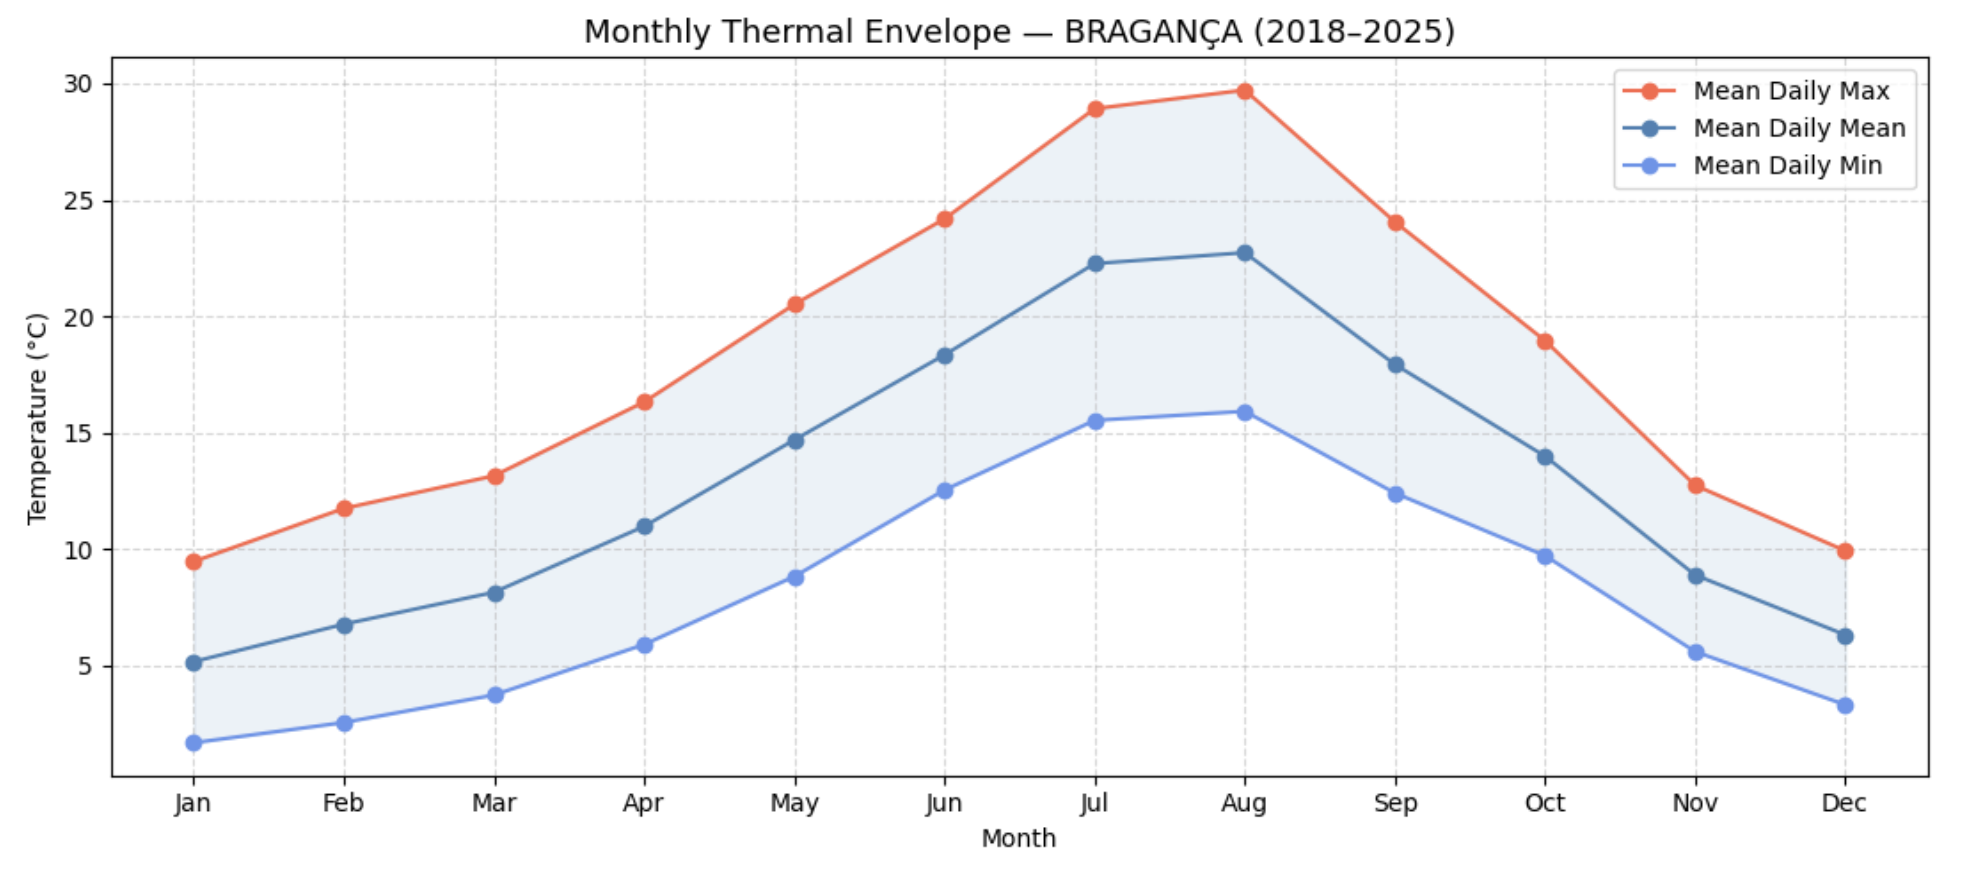
\includegraphics[width=0.9\textwidth]{thermalBraganca.png}
\caption{Monthly thermal envelope (2018–2025) — Bragança}
\label{fig:thermal_br}
\end{figure}

\begin{figure}[H]
\centering
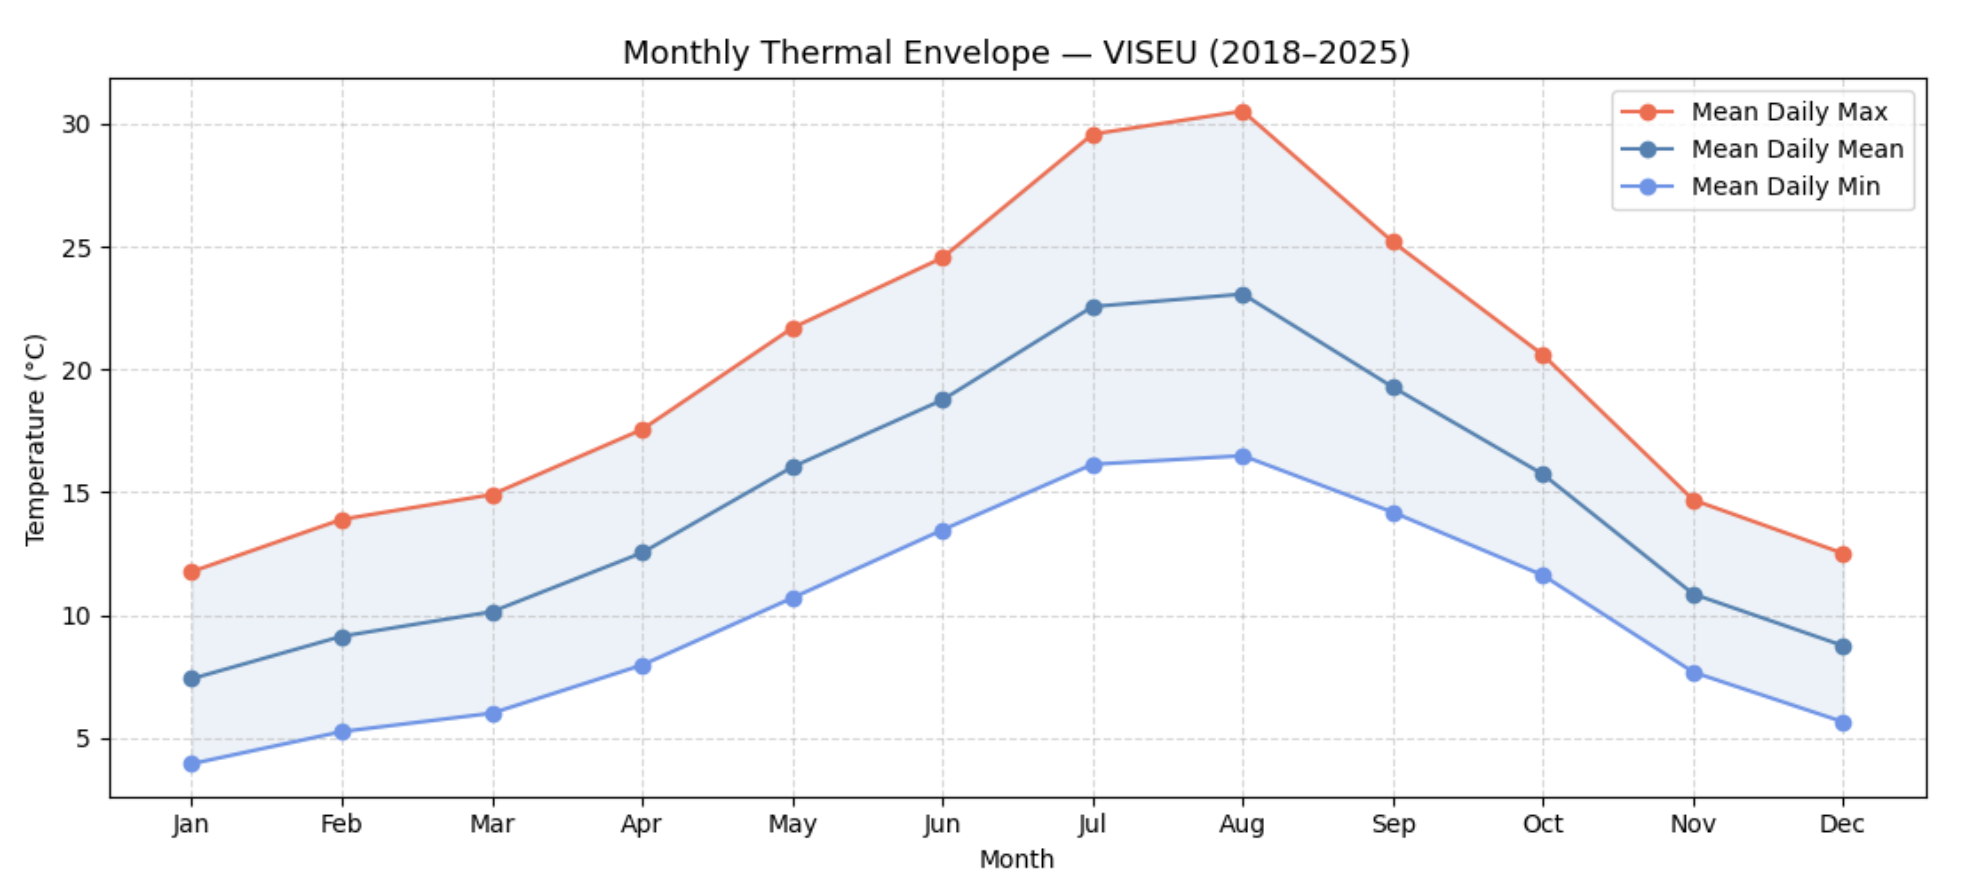
\includegraphics[width=0.9\textwidth]{thermalViseu.png}
\caption{Monthly thermal envelope (2018–2025) — Viseu}
\label{fig:thermal_vi}
\end{figure}

\subsection{Positive Deviations from Monthly Mean Maximum}

The boxplots below show the seasonal distribution of positive deviations — days where the maximum temperature exceeded the monthly mean maximum. These events represent thermal stress periods with elevated cooling demand.

\begin{figure}[H]
\centering
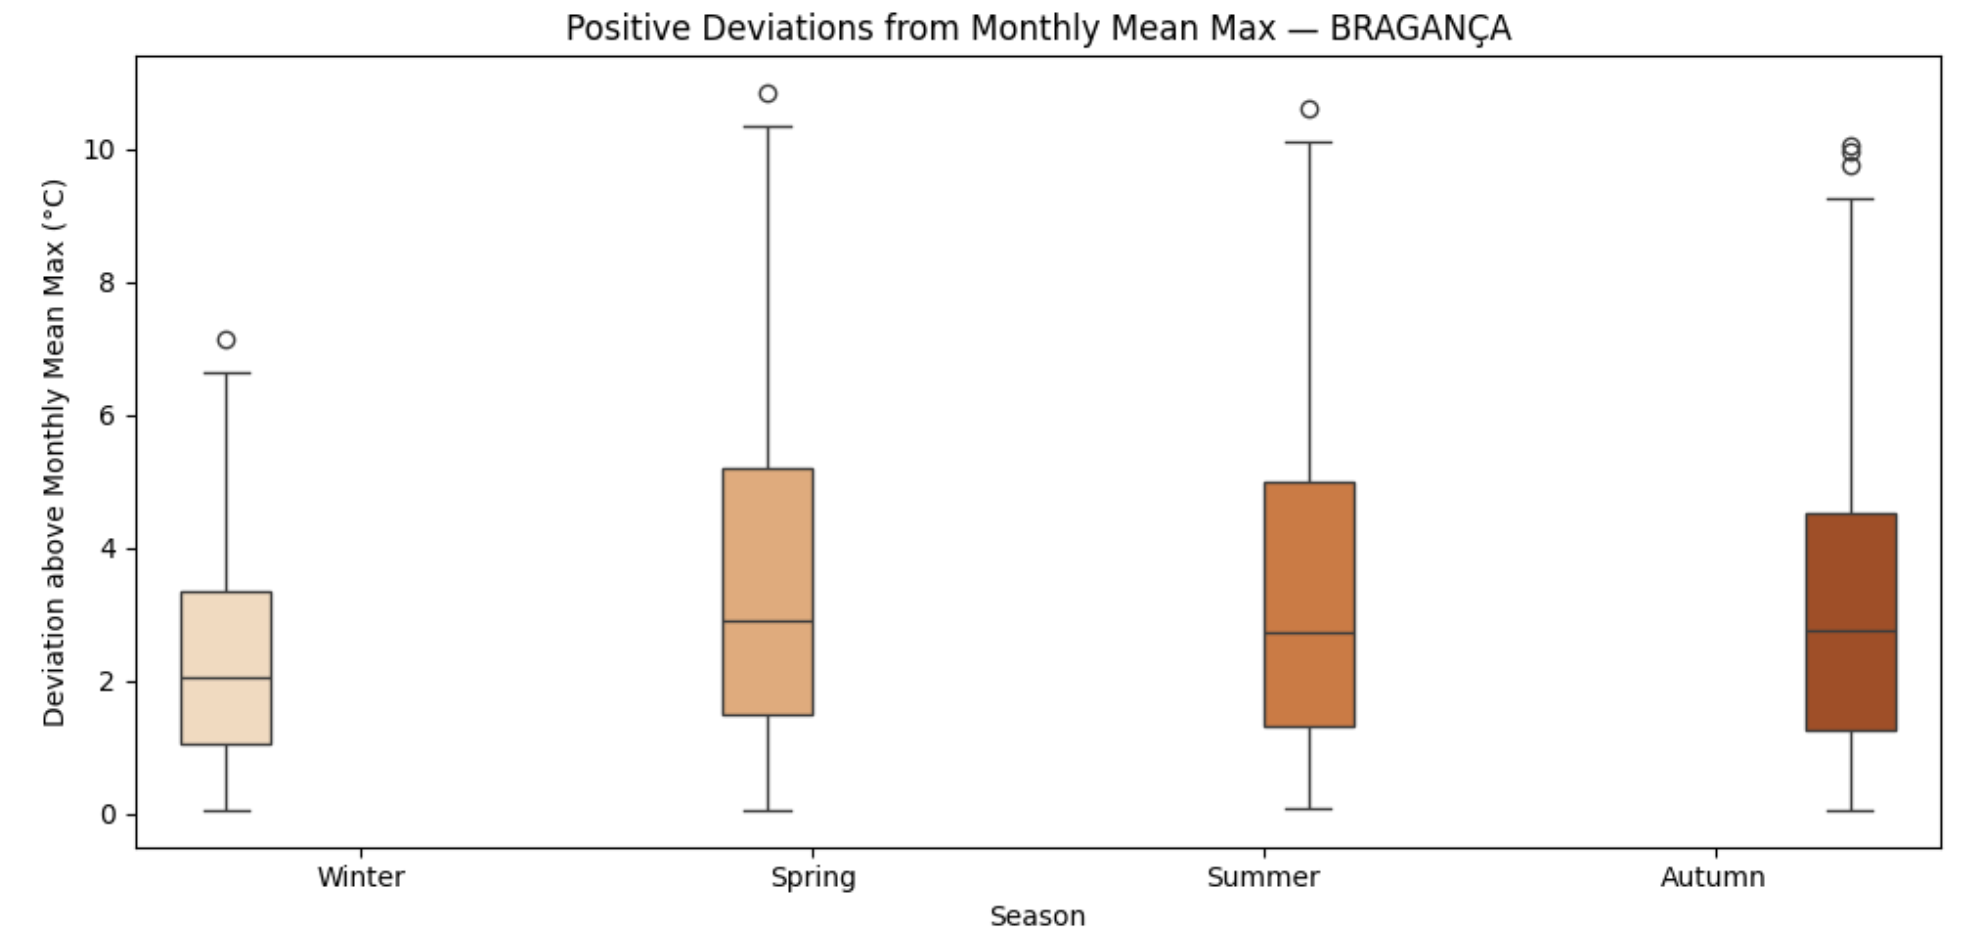
\includegraphics[width=0.85\textwidth]{posDevBrag.png}
\caption{Positive deviations from monthly mean max temperature by season — Bragança}
\label{fig:dev_br}
\end{figure}

\begin{figure}[H]
\centering
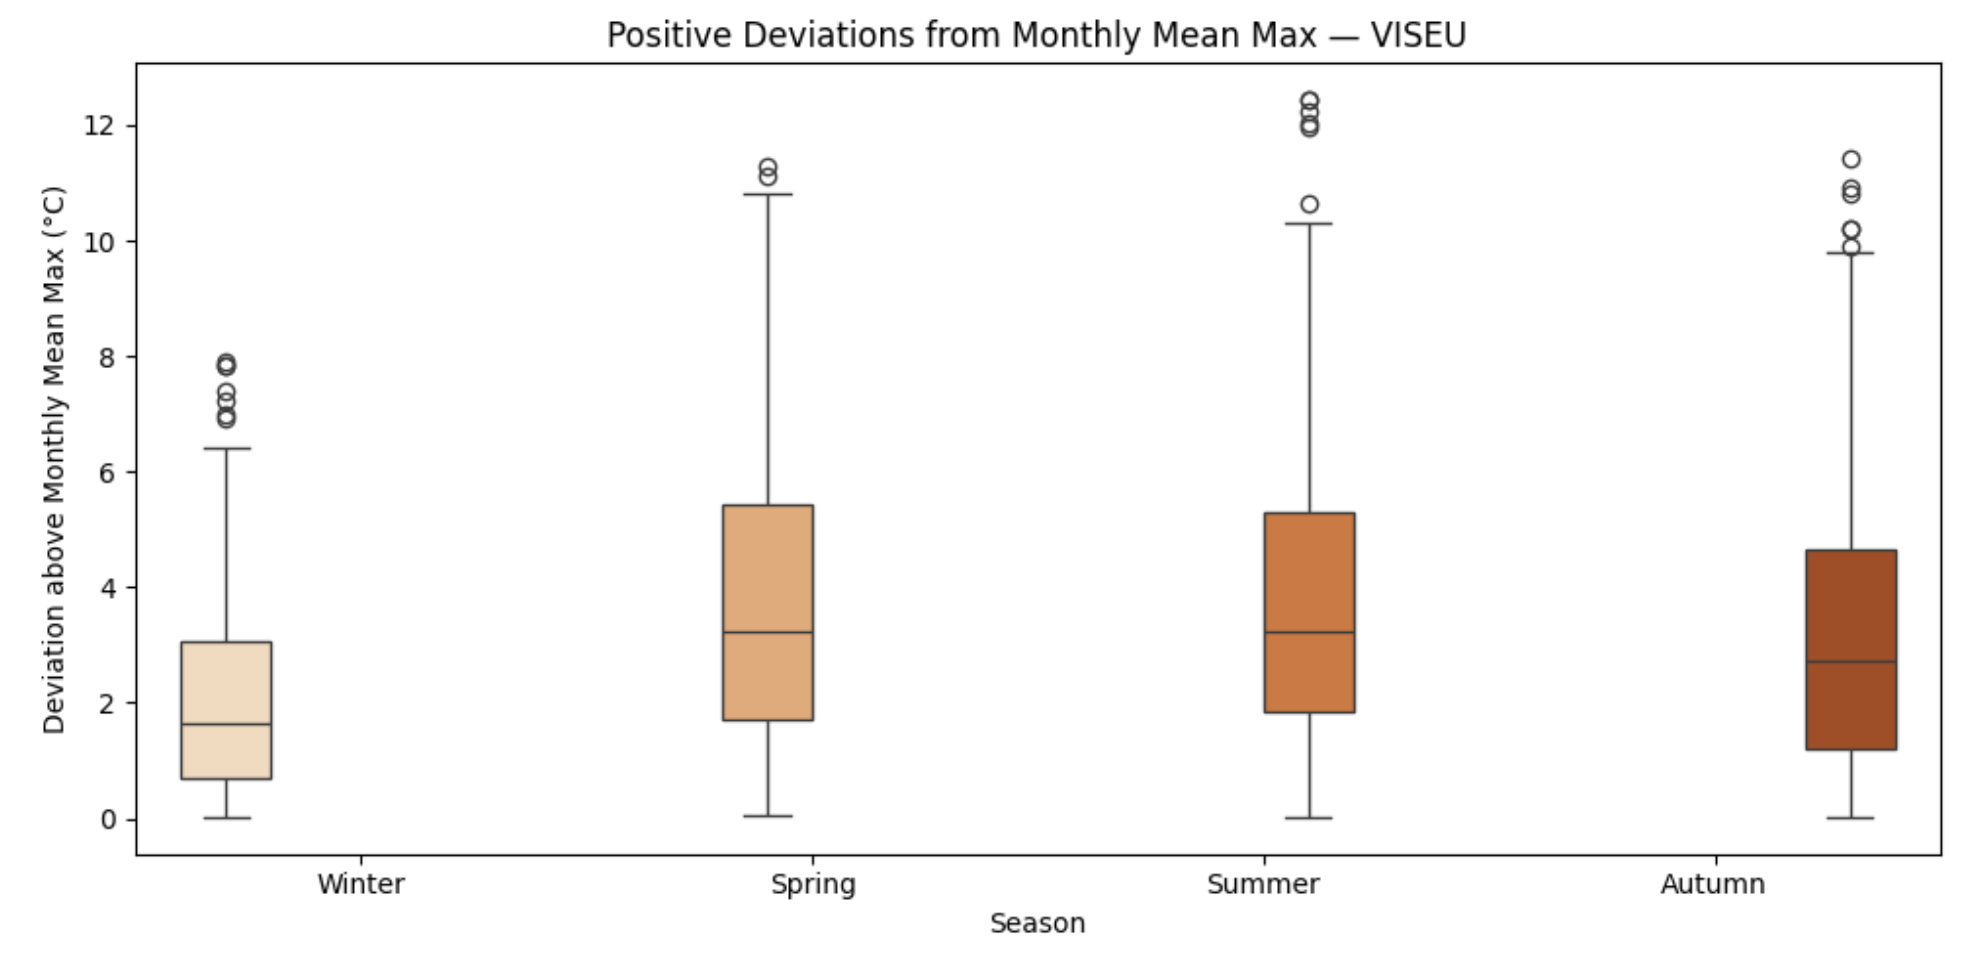
\includegraphics[width=0.85\textwidth]{posDevViseu.png}
\caption{Positive deviations from monthly mean max temperature by season — Viseu}
\label{fig:dev_vi}
\end{figure}

\subsection{Summary Comparison Table}

\begin{table}[H]
\centering
\caption{Head-to-Head Comparison: Bragança vs Viseu}
\label{tab:summary}
\begin{tabular}{lcc}
\toprule
\textbf{Metric} & \textbf{Bragança} & \textbf{Viseu} \\
\midrule
Winter Mean Temp (°C) & 6.07 & 8.41 \\
Summer Mean Temp (°C) & 21.14 & 21.49 \\
Days $\geq$ 25°C & 700 & 786 \\
Days $\geq$ 30°C & 283 & 352 \\
Days $\geq$ 35°C & 35 & 64 \\
Extreme Events (IQR method) & 7 & 6 \\
Summer Stability Index (0–1) & 0.238 & 0.216 \\
Autumn Stability Index (0–1) & 0.293 & 0.333 \\
\bottomrule
\end{tabular}
\end{table}

% =====================================================================================
\section{Discussion}
% =====================================================================================

The analysis reveals a clear and consistent thermal contrast between the two cities. Bragança is colder across every season, with the largest gap occurring in Winter (2.34°C) and Autumn (1.69°C). While summer mean temperatures are nearly identical, Bragança's advantage becomes stark when considering threshold exceedances: it records 45.3\% fewer days above 35°C than Viseu, a critical consideration for the energy efficiency of a cold-storage facility.

The Stability Index tells a more nuanced story. Viseu shows superior stability in Winter and Autumn, reflecting its more maritime-influenced climate. However, Bragança edges ahead in Summer stability (0.238 vs 0.216), which is operationally significant — Summer is when refrigeration demand peaks.

The correlation analysis confirms that solar radiation and humidity are the dominant drivers of temperature and DTR variability. Day length emerges as the strongest single predictor of the Stability Index for both cities, underlining the seasonal structure underlying the data.

Extreme event detection via IQR fences reveals that both cities are largely free from anomalous cold events. Bragança's 7 extreme days cluster in Spring (6 events), while Viseu's 6 events are spread more evenly. Profiling these days confirms they are primarily hot-and-dry anomalies with elevated solar radiation and reduced humidity — consistent with Iberian heat-wave dynamics.

% =====================================================================================
\section{Conclusion}
% =====================================================================================

\textbf{Recommendation: Bragança is the preferred location for the cold-storage logistics facility.}

The key drivers of this recommendation are:

\begin{itemize}
  \item \textbf{Lower mean temperatures across all seasons} — particularly in Winter and Autumn, reducing baseline refrigeration load.
  \item \textbf{Significantly fewer extreme heat days} — 45.3\% fewer days $\geq$35°C and 11\% fewer days $\geq$25°C compared to Viseu.
  \item \textbf{Higher Summer Stability Index} — Bragança's temperature is marginally more predictable during the peak operational season.
  \item \textbf{Lower total thermal load} — fewer cumulative days requiring active cooling above critical thresholds.
\end{itemize}

Viseu's marginal advantages — slightly superior Winter and Autumn thermal stability, and one fewer IQR-defined extreme event — do not outweigh Bragança's clear edge in overall thermal load and high-temperature frequency. From a logistics and energy cost perspective, Bragança offers the more favorable climate profile.

\end{document}
